\documentclass{article}
\usepackage[utf8]{inputenc}

\title{Outcome Prediction of League of Legends Diamond Ranked Games}
\author{Machao Deng, Zining Ma}
\date{April 28th, 2020}

\usepackage{natbib}
\usepackage{graphicx}
\usepackage{fpstyle}

\begin{document}

\maketitle

\section{Abstract}
The League of Legends Diamond Ranked Games dataset contains approximate 10000 observations and 40 variables. The dataset is available on kaggle \cite{kaggledata}. In this project,we applied Gaussian process, support vector machine, and neural network to predict the wining side of a game, and compare the behavior of each algorithm.

\section{Introduction}
League of Legends (LoL) is a multiplayer online battle arena video game developed and published by Riot Games. In League of Legends, players assume the role of a "champion" with unique abilities and battle against a team of other player or computer-controlled champions. The goal is usually to destroy the opposing team's "Nexus", a structure that lies at the heart of a base protected by defensive structures.

The dataset contains the first ten minutes information of each game at "diamond" ranking, which is a very high competitive level in the LoL. The reason for only choosing diamond ranking games is because the players in this level are less likely to make faults, which proves the objectivity of data and decrease the negative affection brought by the players.

The dataset includes nearly 10000 observations and 40 features that record the information for the blue and red team of each game. In this project, we are going to divide the dataset into train and test set. We plan to build several machine learning models we have learned in this class based on train set and assess our models on the test set. Another purpose is to find the difference among the the different models.

\subsection{Variable Explanation}

The data include:

$\bullet$ Unique RIOT ID of the game.

$\bullet$ The target column. 1 if the blue team has won, 0 otherwise.

$\bullet$ Number of warding totems placed by the blue or red team on the map

$\bullet$ Number of enemy warding totems the blue or red team has destroyed

$\bullet$ First kill of the game. 1 if the blue team did the first kill, 0 otherwise

$\bullet$ Number of enemies killed by the blue or red team

$\bullet$ Number of deaths (blue or red team)

$\bullet$ Number of kill assists (blue or red team)

$\bullet$ Number of elite monsters killed by the blue or red team (Dragons and Heralds)

$\bullet$ Number of dragons killed by the blue or red team

$\bullet$ Number of heralds killed by the blue or red team

$\bullet$ Blue or red team total gold

$\bullet$ Blue or red team average champion level

$\bullet$ Blue or red team total experience

$\bullet$ Blue or red team total minions killed (CS)

$\bullet$ Blue or red team total jungle monsters killed

$\bullet$ Blue team gold difference compared to the enemy team

$\bullet$ Blue team experience difference compared to the enemy team

$\bullet$ Blue or red team CS (minions) per minute

$\bullet$ Blue or red team gold per minute

\section{Methods and Results}

\subsection{Gaussian Process}
The Gaussian Process Classifier uses Bayes Theorem to extrapolate the posterior probability $P(C_{k}|x)$, where $C_{k}$ represents class k and $x$ is a featured vector that has a Gaussian (univariate or multivariate) prior. Gaussian Process is that we can place priors over parameters using a kernel and evaluate the variance of parameters. During the Gaussian Process, the different kernel will give us different outcomes.

For this dataset, we first delete some duplicated information such as "blue team gold difference" and "red team gold difference" since they actually represent the same thing. Then, we choose the first 8000 observations as train data and the rest of the observations as test data. We build our Gaussian Process model on train data, treating the variable "blueWins" as the target variable and the rest of features as train variables. In the mean time, we have tried many different kernels for this problem and we find out Radial-basis function (RBF) works best. Finally, the accuracy on test set is 72.1\%.

\subsection{Support Vector Machine}
Support vector machines (SVMs) are a set of supervised learning methods used for classification, regression and outliers detection. It is a linear classifier that, given data in $R^p$, finds the hyperplane which has the greatest margins to the data points. The hyperplane is defined as:
$$ argmin_{w,b,\epsilon}(\frac{1}{2}||w||^2+C\sum_{i=1}^{n}\epsilon_{i}), \space y_{i}(w \cdot x_{i}+b)\ge 1-\epsilon_{i},\space \forall i, $$

where $\epsilon_{i}$ is the penalty for misclassification. There also exists non-linear SVM which maps the data points into high dimensional space first, and then uses kernel function to get a dot product in that space.

The setting is the same as the previous one. The linear and Rbf kernel are both well-behaved. The accuracy on test set are 71.6\% and 72.5\% respectively.

\subsection{Neural Network}
We tried 8 different neural network structures to do the classification considering choices of activation functions, layer width, network depth and batch normalization. The structures of networks is shown in Table 1.

\begin{table}[h!]
\caption{Network structures}
\centering
\begin{tabular}{ |p{2cm}|p{2cm}|p{2cm}|p{3.2cm}|  }
\hline
Structure 1& Structure 2 &Structure 3 & Structure 4 \\
\hline
Input & Input & Input & Input \\
Dense(64) & Dense(128) & Dense(64) & Dense(64) \\
Dense(64) & Dense(128) & Dense(64) & BatchNormalization \\
Dense(64) & Dense(128) & Dense(64) & Dense(64) \\
Dense(64) & Dense(128) & Dense(64) & BatchNormalization \\
Output & Output & Dense(32) & Dense(64) \\
 &  & Dense(32) & BatchNormalization \\
 &  & Dense(32) & Dense(64) \\
 &  & Dense(32) & BatchNormalization \\
 &  & Output & Output \\
\hline
\end{tabular}
\end{table}

The data we used is as same as in above methods. For all networks, we trained them adam optimizer and set crossentropy as loss function. All models are trained for 100 epoches.

\begin{figure}[h!]
\centering
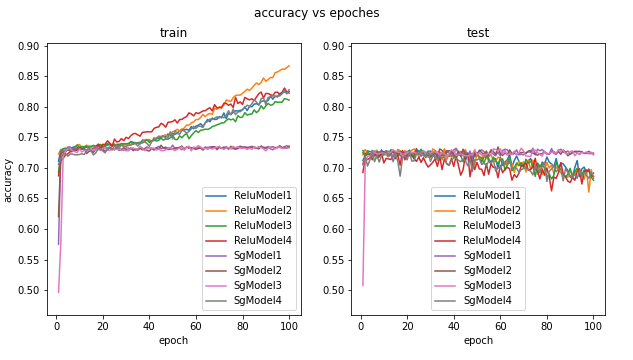
\includegraphics[scale=0.8]{accuracy.png}
\caption{Plot of accuracy vs epoch for 8 models. A model with structure 1 and relu as activation function is named ReluModel1, and a model with structure 2 and sigmoid as activation function is named SgModel1, etc.}
\label{fig:universe}
\end{figure}


Figure 1. shows how train and test accuracy vary with epoches. We can see that before 20 epoches, all networks converged to same accuray on both train and test set respectively. However, after 20 epoches, overfitting happens on all ReLu models and Sigmoid model 4. The result tells that a shallow network with sigmoid activation function is stable for this problem. Besides, We didn't observed significant difference before overfitting among these structures. Mean and std of test accuracy of 8 models among $10\sim 20$ epoches are shown in Table 2. The highest test accuracy we obtained is 73.4\% by SgModel2.

\begin{table}[h!]
\caption{Test accuracy}
\centering
\begin{tabular}{ |p{2cm}||p{2cm}|p{2cm}|p{2cm}|p{2cm}|  }
\hline
Activation & Structure 1& Structure 2 &Structure 3 & Structure 4 \\
\hline
ReLu & 72.4\%(0.3\%) & 72.4\%(0.4\%) & 72.4\%(0.3\%) & 71.6\%(0.6\%) \\
\hline 
sigmoid & 72.4\%(0.2\%) & 72.4\%(0.2\%) & 72.4\%(0.2\%) & 71.4\%(1.0\%) \\
\hline
\end{tabular}
\end{table}

\section{Discussion and Conclusion}

In this problem, we tried 3 different methods, Gaussian process, support vector machine and neural network to predict winner of a game set using statistics from first 10 minutes. Consequently, all three methods performs similarly on test set, achieving test accuracy at $71\%\sim73\%$. The result may suggest that statistics from first 10 minutes could only give $71\%\sim73\%$ of decisive information of a game. In other words, more information is necessary to achieve an accuracy above $73\%$.

When we were training Gaussian process model, we found that choice of kernel function and parameter is significant. We tried RBF and other kernels such as Matern, RationalQuadratic, DotProduct and ExpSineSquared, and trained with different initial parameters. An inappropriate kernel could result in $50\%$ test accuracy which is the same as random prediction. The one we report in methods is the one performed best on test set. The phenomena tells that an appropriate space (corresponding to a kernel) to embed data is significant in training Gaussian process model.

The results of neural network suggested that in comparison of deep network with relu activation function and applying batch normalization, a shallow network with sigmoid activation function works more stable in this problem. However, this stability could also be a result of slow convergence of network using sigmoid function. We didn't observed overfitting in 100 epoches in SgModels 1,2 and 3. However, the overfitting of SgModel 4, a sigmoid network with batch normalization which could accelerate training speed, may suggest that overfitting will happen in more epoches.


\bibliographystyle{plain}
\bibliography{references}
\end{document}
